%-----------------------------------------------------------------------------
%
%               Template for sigplanconf LaTeX Class
%
% Name:         sigplanconf-template.tex
%
% Purpose:      A template for sigplanconf.cls, which is a LaTeX 2e class
%               file for SIGPLAN conference proceedings.
%
% Author:       Paul C. Anagnostopoulos
%               Windfall Software
%               978 371-2316
%               paul@windfall.com
%
% Created:      15 February 2005
%
%-----------------------------------------------------------------------------


\documentclass{sigplanconf}

% The following \documentclass options may be useful:
%
% 10pt          To set in 10-point type instead of 9-point.
% 11pt          To set in 11-point type instead of 9-point.
% authoryear    To obtain author/year citation style instead of numeric.

\usepackage{microtype}
\usepackage{ifthen}
\usepackage{fancyvrb}
\usepackage{color}
\usepackage{ulem}
\usepackage{xspace}
\usepackage{epsfig}
\usepackage{amssymb}
\usepackage{amsmath}
\usepackage{amsfonts}
\usepackage[utf8]{inputenc}
\usepackage{setspace}
\usepackage{relsize}

\usepackage{listings}

\usepackage[T1]{fontenc}
\usepackage{setspace}
\usepackage{listings}
\usepackage[scaled=0.81]{beramono}

\definecolor{gray}{rgb}{0.3,0.3,0.3}

\lstset{
  basicstyle=\setstretch{1.05}\ttfamily\footnotesize,
  language=Python,
  keywordstyle=\bfseries,
  stringstyle=\color{blue},
  commentstyle=\color{gray}\textit,
  fancyvrb=true,
  showstringspaces=false,
  %keywords={def,while,if,elif,return,class,get,set,new,guard_class}
  numberstyle = \tiny,
  numbersep = -20pt,
}


\newboolean{showcomments}
\setboolean{showcomments}{true}
\ifthenelse{\boolean{showcomments}}
  {\newcommand{\nb}[2]{
    \fbox{\bfseries\sffamily\scriptsize#1}
    {\sf\small$\blacktriangleright$\textit{#2}$\blacktriangleleft$}
   }
   \newcommand{\version}{\emph{\scriptsize$-$Id: main.tex 19055 2008-06-05 11:20:31Z cfbolz $-$}}
  }
  {\newcommand{\nb}[2]{}
   \newcommand{\version}{}
  }

\newcommand\cfbolz[1]{\nb{CFB}{#1}}
\newcommand\arigo[1]{\nb{AR}{#1}}
\newcommand\fijal[1]{\nb{FIJAL}{#1}}
\newcommand\david[1]{\nb{DAVID}{#1}}
\newcommand\anto[1]{\nb{ANTO}{#1}}
\newcommand\hakan[1]{\nb{HAKAN}{#1}}
\newcommand\reva[1]{\nb{Reviewer 1}{#1}}
\newcommand\revb[1]{\nb{Reviewer 2}{#1}}
\newcommand\revc[1]{\nb{Reviewer 3}{#1}}
\newcommand\revd[1]{\nb{Reviewer 4}{#1}}
\newcommand{\commentout}[1]{}
\newcommand{\ignore}[1]{} % {{\tt \small ignore(#1)}}

\newcommand\ie{i.e.,\xspace}
\newcommand\eg{e.g.,\xspace}
\newcommand{\etal}{\emph{et al.}\xspace}

\normalem

\let\oldcite=\cite

\renewcommand\cite[1]{\ifthenelse{\equal{#1}{XXX}}{[citation~needed]}{\oldcite{#1}}}


\begin{document}

\conferenceinfo{DLS'12,} {October 22, 2012, Tucson, Arizona, USA.}
\CopyrightYear{2012}
\copyrightdata{978-1-4503-1564-7/12/10}

\titlebanner{draft}        % These are ignored unless
%\preprintfooter{short description of paper}   % 'preprint' option specified.

\title{Loop-Aware Optimizations in PyPy's Tracing JIT}
%\subtitle{Subtitle Text, if any}

\authorinfo{H\aa kan Ardö}
           {Centre for Mathematical Sciences, Lund University}
           {hakan@debian.org}
\authorinfo{Carl Friedrich Bolz}
           {Heinrich-Heine-Universität Düsseldorf}
           {cfbolz@gmx.de}
\authorinfo{Maciej Fijałkowski}
           {}
           {fijall@gmail.com}

\maketitle

\begin{abstract}
One of the nice properties of a tracing just-in-time compiler (JIT) is that many of its optimizations
are simple, requiring one forward pass only. This is not true for loop-invariant code
motion which is a very important optimization for code with tight kernels.
Especially for dynamic languages that typically perform quite a lot of loop invariant
type checking, boxed value unwrapping and virtual method lookups.

In this paper we explain a scheme pioneered within the context of the LuaJIT project
for making basic optimizations loop-aware by
using a simple pre-processing step on the trace without changing the
optimizations themselves.

We have implemented the scheme in RPython's tracing JIT compiler. PyPy's Python
JIT executing simple numerical kernels can become up to two times faster,
bringing the performance into the ballpark of static language compilers.
\end{abstract}

\category{D.3.4}{Programming Languages}{Processors}[code generation,
incremental compilers, interpreters, run-time environments]

\terms
Languages, Performance, Experimentation

\keywords{Tracing JIT, Optimization, Loop-Invariant Code Motion}

\section{Introduction}

A dynamic language typically needs to do quite a lot of type
checking, wrapping/unwrapping of boxed values, and virtual method dispatching. 
For tight computationally intensive loops a
significant amount of the execution time might be spent on such tasks
instead of the actual computations. Moreover, the type checking,
unwrapping and method lookups are often loop invariant and performance could be increased
by moving those operations out of the loop. We explain a simple scheme
to make a tracing JIT loop-aware by allowing it's existing optimizations to
perform loop invariant code motion. 

One of the advantages that tracing just-in-time compilers (JITs) have above traditional
method-based
JITs is that their optimizers are much easier to write. Because a tracing JIT
produces only linear pieces of code without control flow joins, many
optimization passes on traces can have a very simple structure: They often
consist of one forward pass replacing operations by faster ones or even
discarding them as they walk along it. This makes
optimization of traces very similar to symbolic execution. Also, many
difficult problems in traditional optimizers become tractable if the optimizer
does not need to deal with control flow merges.

One disadvantage of this simplicity is that such forward-passing
optimizers ignore the only bit of control flow they have available, which is
the fact that most traces actually represent loops. Making use of this
information is necessary to perform optimizations that take the whole loop into
account, such as loop-invariant code
motion or optimizations that improve several iterations of the loop.
Having to deal with this property of traces complicates the optimization passes,
as a more global view of a trace needs to be considered when optimizing.

Mike Pall pioneered a solution to address this problem in the context of a
dynamic language using a tracing JIT compiler. He published his algorithm and
its rationale in 2009~\cite{pall_luajit_2009} and implemented it in LuaJIT
2.0\footnote{\texttt{http://luajit.org/}}, an open source JIT compiler for the Lua
language. His approach allows to reuse all forward pass
optimizations to achieve loop invariant code motion and other loop-related
optimizations, which greatly simplifies the implementation. We have implemented
the same approach in RPython's tracing JIT compiler, the results of which we
present here.

The resulting optimizations one gets using this scheme are in no way novel, most
of them are well-known loop optimizations. However, the way to implement them is
a lot simpler than directly implementing loop-aware optimizations.

% loop peeling does a lot more than loop-invariant code motion
% take this loop as an example:
% [i1, i2]
% i3 = i1 + 1
% i4 = i2 + 1
% escape(i4)
% jump(i2, i3)
% none of the operations is loop-invariant, but loop peeling will still remove the second addition

\section{Background: RPython and PyPy}
\label{sec:PyPy}

The work described in this paper was done in the context of the PyPy
project.\footnote{\texttt{http://pypy.org}} PyPy is a framework for implementing
dynamic languages efficiently~\cite{rigo_pypys_2006}. When implementing a
language with PyPy, one writes an interpreter for the language in RPython~\cite{ancona_rpython:_2007}.
RPython (``Restricted Python``) is a subset
of Python chosen in such a way that it can be efficiently translated to a
C-based virtual machine (VM) by performing type inference.

Many low-level aspects of the final VM are not contained within the interpreter
implementation but are inserted during translation to C. Examples for this are a
garbage collector and also a tracing JIT compiler~\cite{bolz_tracing_2009}.

RPython's tracing JIT compiler traces on the level of RPython programs. Thus it
actually traces the execution of an interpreter written in RPython, not of the
program itself. This makes the details of the object model of the implemented
language transparent and optimizable by the tracing JIT. In the context of this
paper, this aspect of RPython's tracing JIT can be ignored. Instead, it is
sufficient to view RPython's tracing JIT as a JIT for RPython.


% section PyPy (end)

\section{Motivation}
\label{sec:Motivation}

To motivate the approach we propose here, let's look at a trivial (unrealistic)
trace which corresponds to an infinite loop:


\begin{lstlisting}[mathescape,numbers = right,basicstyle=\setstretch{1.05}\ttfamily\scriptsize]
$L_0$($i_{0}$):
$i_1$ = $i_0$ + 1
print($i_1$)
jump($L_0$, $i_0$)
\end{lstlisting}

The first line is a label $L_0$ with argument $i_0$. Every label has a list of
arguments. The \lstinline{print} operation just prints its argument (it is not
an operation that RPython's tracing JIT really supports, we just use it for this
example). The \lstinline{jump} operation jumps back to the beginning of the
trace, listing the new values of the arguments of the trace. In this case, the
new value of $i_0$ is $i_0$, making it a loop-invariant.

Because $i_0$ is loop-invariant, the addition could be moved out of the loop.
However, it is desirable to get this effect using our existing optimization passes
without changing them too much. Optimizations with one forward pass
cannot directly achieve this effect: They just look at the trace without taking
into account that the trace executes many times in a row. Therefore to achieve
loop-invariant code motion, we peel one iteration off the loop before running
the optimizations. This peeling gives the following trace:

\begin{lstlisting}[mathescape,numbers = right,basicstyle=\setstretch{1.05}\ttfamily\scriptsize]
$L_0$($i_{0}$):
$i_1$ = $i_0$ + 1
print($i_1$)
jump($L_1$, $i_0$)

$L_1$($i_{0}$):
$i_2$ = $i_0$ + 1
print($i_2$)
jump($L_1$, $i_0$)
\end{lstlisting}

The iteration of the loop that was peeled off (lines 1-4) is called the
\emph{preamble}, the loop afterwards (lines 6-9) the \emph{peeled loop}.

Now the optimizer optimizes both of these two iterations of the loop together,
disregarding the \lstinline{jump} and the label in lines 4-6. Doing this, common
subexpression elimination will discover that the two additions are the same, and
replace $i_2$ with $i_1$. This leads to the following trace:

\begin{lstlisting}[mathescape,numbers = right,basicstyle=\setstretch{1.05}\ttfamily\scriptsize]
$L_0$($i_{0}$):
$i_1$ = $i_0$ + 1
print($i_1$)
jump($L_1$, $i_0$)

$L_1$($i_{0}$):
print($i_1$)
jump($L_1$, $i_0$)
\end{lstlisting}

This trace is malformed, because $i_1$ is used after the label $L_1$ without
being passed there, so we need to add $i_1$ as an argument to the label and pass
it along the \lstinline{jump}s:

\begin{lstlisting}[mathescape,numbers = right,basicstyle=\setstretch{1.05}\ttfamily\scriptsize]
$L_0$($i_{0}$):
$i_1$ = $i_0$ + 1
print($i_1$)
jump($L_1$, $i_0$, $i_1$)

$L_1$($i_{0}$, $i_1$):
print($i_1$)
jump($L_1$, $i_0$, $i_1$)
\end{lstlisting}

The final result is that the loop-invariant code was moved out of the loop into
the peeled-off iteration. Thus the addition is only executed in the first
iteration, while the result is reused in all further iterations.

This scheme is quite powerful and generalizes to other optimizations than just
common subexpression elimination. It allows linear optimization passes to
perform loop-aware optimizations, such as loop-invariant code motion without
changing them at all. All that is needed is to peel off one iteration, then
apply one-pass optimizations and make sure that the necessary extra
arguments are inserted into the label of the loop itself and the jumps
afterwards.

This is the key insight of the implementation scheme: If an
optimization is given two iterations together at the same time, the
optimization has enough context to remove operations from the peeled loop,
because it detects
that the operation was performed in the preamble already. Thus at runtime these
moved operations are only executed once when entering the loop and the results
are reused in further iterations.


% section Motivation (end)

\section{Running Example}
\label{sub:example}

The last section gave a motivating but unrealistically small example.
This section will define a slightly larger example that the rest of the paper
uses to demonstrate the effect of optimizations.
For this we are going to use a tiny interpreter for a dynamic language with
 a very small object
model, that just supports an integer and a float type (this example has been taken from a previous paper~\cite{bolz_allocation_2011}). The objects support only
one operation, \lstinline{add}, which adds two objects (promoting ints to floats in a
mixed addition). The implementation of \lstinline{add} uses classical
double-dispatching.
%These classes could be part of the implementation of a very
%simple interpreter written in RPython.
The classes can be seen in
Figure~\ref{fig:objmodel} (written in RPython).

\begin{figure}
\begin{lstlisting}[mathescape,basicstyle=\setstretch{1.05}\ttfamily\scriptsize]
class Base(object):
   pass

class BoxedInteger(Base):
   def __init__(self, intval):
      self.intval = intval

   def add(self, other):
      return other.add__int(self.intval)

   def add__int(self, intother):
      return BoxedInteger(intother + self.intval)

   def add__float(self, floatother):
      floatvalue = floatother + float(self.intval)
      return BoxedFloat(floatvalue)


class BoxedFloat(Base):
   def __init__(self, floatval):
      self.floatval = floatval

   def add(self, other):
      return other.add__float(self.floatval)

   def add__int(self, intother):
      floatvalue = float(intother) + self.floatval
      return BoxedFloat(floatvalue)

   def add__float(self, floatother):
      return BoxedFloat(floatother + self.floatval)


def f(y):
   step = BoxedInteger(-1)
   while True:
      y = y.add(step)
\end{lstlisting}
\caption{An ``Interpreter'' for a Tiny Dynamic Language Written in RPython}
\label{fig:objmodel}
\end{figure}

Using these classes to implement arithmetic shows the basic problem of many
dynamic language implementations. All the numbers are instances of either
\lstinline{BoxedInteger} or \lstinline{BoxedFloat}, therefore they consume space on the
heap. Performing many arithmetic operations produces lots of garbage quickly,
putting pressure on the garbage collector. Using double dispatching to
implement the numeric tower needs two method calls per arithmetic operation,
which is costly due to the method dispatch.

Let us now consider an ``interpreter'' function \lstinline{f} that uses the
object model (see the bottom of Figure~\ref{fig:objmodel}).
Simply running this function is slow, because there are lots of virtual method
calls inside the loop, two for each
call to \lstinline{add}. These method calls need to check the type of the involved
objects every iteration. In addition, a lot of objects are created
when executing that loop, many of these objects are short-lived.
The actual computation that is performed by \lstinline{f} is simply a sequence of
float or integer additions (note that \lstinline{f} does not actually terminate,
but it is still instructive to look at the produced traces).


\begin{figure}
\begin{lstlisting}[mathescape,numbers = right,basicstyle=\setstretch{1.05}\ttfamily\scriptsize]
$L_0$($p_{0}$, $p_{1}$):
# inside f: y = y.add(step)
guard_class($p_{1}$, BoxedInteger)
    # inside BoxedInteger.add
    $i_{2}$ = get($p_{1}$, intval)
    guard_class($p_{0}$, BoxedInteger)
        # inside BoxedInteger.add__int
        $i_{3}$ = get($p_{0}$, intval)
        $i_{4}$ = $i_{2} + i_{3}$
        $p_{5}$ = new(BoxedInteger)
            # inside BoxedInteger.__init__
            set($p_{5}$, intval, $i_{4}$)
jump($L_0$, $p_{0}$, $p_{5}$)
\end{lstlisting}
\caption{An Unoptimized Trace of the example interpreter}
\label{fig:unopt-trace}
\end{figure}

If the function is executed using the tracing JIT, with \lstinline{y} being a
\lstinline{BoxedInteger}, the produced trace looks like the one of
Figure~\ref{fig:unopt-trace} (lines starting with a hash ``\#'' are comments).
The trace corresponds to one iteration of the while-loop in \lstinline{f}.

The operations in the trace are indented
corresponding to the stack level of the function that contains the traced
operation. The trace is in single-assignment form, meaning that each variable is
assigned a value exactly once. The arguments $p_0$ and $p_1$ of the loop correspond
to the live variables \lstinline{y} and \lstinline{step} in the while-loop of
the original function.

The label of the loop is $L_0$ and is used by the jump instruction to
identify it's jump target.

The operations in the trace correspond to the operations in the RPython program
in Figure~\ref{fig:objmodel}:

\begin{itemize}
    \item \lstinline{new} creates a new object.
    \item \lstinline{get} reads an attribute of an object.
    \item \lstinline{set} writes to an attribute of an object.
    \item \lstinline{guard_class} is a precise type check, not checking for subclasses.
\end{itemize}

Inlined method calls in the trace are preceded by a \lstinline{guard_class}
operation, to check that the class of the receiver is the same as the one that
was observed during tracing. These guards make the trace specific
to the situation where \lstinline{y} is really a \lstinline{BoxedInteger}. When
the trace is turned into machine code and afterwards executed with
\lstinline{BoxedFloat}, the
first \lstinline{guard_class} instruction will fail and execution will continue
using the interpreter.

\section{Making Trace Optimizations Loop Aware}

Before a trace is compiled to machine code by the backend,
it is optimized to achieve better performance.
One goal of that is to move 
operations out of the loop to execute them only once
and not every iteration. This can be achieved by loop peeling. It
leaves the loop body intact, but prefixes it with one iteration of the
loop. This operation by itself will not achieve anything. But if it is
combined with other optimizations it can increase the effectiveness of
those optimizations. For many optimizations of interest only a few
additional details have to be considered when they are combined with loop peeling. These are
described below by explaining the loop peeling optimization
followed by a set of other optimizations and how they interact with
loop peeling.

\subsection{Loop Peeling}

\begin{figure}
\begin{center}
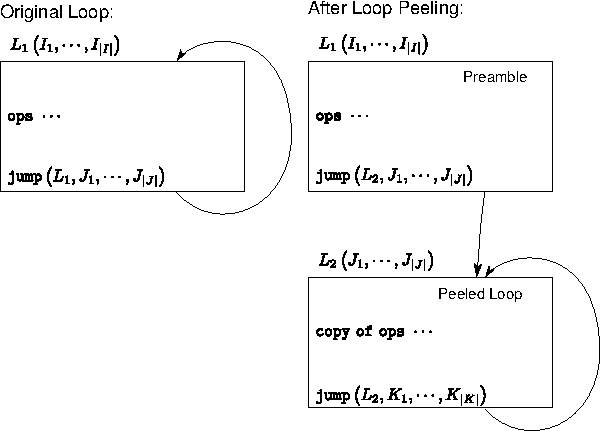
\includegraphics[width=\columnwidth]{figures/overview}
\end{center}
\caption{Overview of Loop Peeling}
\label{fig:overview}
\end{figure}

Loop peeling is achieved by appending a copy of the traced iteration at
the end of itself. See Figure~\ref{fig:overview} for an illustration.
The first part (called \emph{preamble}) finishes with a jump to the second part
(called the \emph{peeled loop}). The second part finishes with a jump to itself. This way
the preamble will be executed only once while the peeled loop will
be used for every further iteration. New variable names have to be
introduced in the entire copied trace in order to maintain the SSA-property.

When peeling the loop, no assumptions are made that the preamble is
the \emph{first} iteration, when later executing the loop. The preamble stays
general enough to correspond to any iteration of the loop.
However, the peeled loop can then be optimized using the assumption that a
previous iteration (the preamble) has been executed already.

%XXX (samuele): the point about the first iteration is hard to understand

When applying optimizations to this two-iteration trace
some care has to taken as to how the arguments of the two
\lstinline{jump} operations and the input arguments of the peeled loop are
treated. It has to be ensured that the peeled loop stays a proper
trace in the sense that the operations within it only operate on
variables that are either among its input arguments 
or produced within the peeled loop. To ensure this we need
to introduce a bit of formalism.

The original trace (prior to peeling) consists of three parts.
A vector of input
variables, $I=\left(I_1, I_2, \cdots, I_{|I|}\right)$, a list of non-
jump operations and a single
jump operation. The jump operation contains a vector of jump variables,
$J=\left(J_1, J_2, \cdots, J_{|J|}\right)$, that are passed as the input variables of the target loop. After
loop peeling there will be a second copy of this trace with input
variables equal to the jump arguments of the preamble, $J$, and jump
arguments $K$. 
Figure~\ref{fig:overview} illustrates the general case. The running
example in Figure~\ref{fig:unopt-trace} has  $I = \left( p_0, p_1
\right)$ and $J = \left( p_0, p_5 \right)$. The result of applying
loop peeling to it is shown in Figure~\ref{fig:peeled-trace} with 
$K = \left( p_0, p_9 \right)$. 

To construct the second copy of the trace (the peeled loop) from the
first (the preeamble) we need a
function $m$, mapping the variables of the preamble onto the
variables of the peeled loop. This function is constructed during the
copying. It is initialized by mapping the input arguments, $I$, to
the jump arguments $J$,
\begin{equation}
  m\left(I_i\right) = J_i \ \text{for}\ i = 1, 2, \cdots |I| .
\end{equation}
In the example that means:

\begin{equation}
  %\left\{
    \begin{array}{lcl}
      m\left(p_0\right) &=& p_0 \\
      m\left(p_1\right) &=& p_5
    \end{array}
  %\right.
  .
\end{equation}



Each operation in the trace is copied in order.
To copy an operation $v=\text{op}\left(A_1, A_2, \cdots, A_{|A|}\right)$
a new variable, $\hat v$, is introduced. The copied operation will
return $\hat v$ using
\begin{equation}
  \hat v = \text{op}\left(m\left(A_1\right), m\left(A_2\right), 
    \cdots, m\left(A_{|A|}\right)\right) . 
\end{equation}
Before the
next operation is copied, $m$ is extend by assigning $m\left(v\right) = \hat
v$. For the example above, that will extend $m$ with
\begin{equation}
  %\left\{
    \begin{array}{lcl}
      m\left(i_2\right) &=& i_6 \\
      m\left(i_3\right) &=& i_7 \\
      m\left(i_4\right) &=& i_8 \\
      m\left(p_5\right) &=& p_9 \\
    \end{array}
  %\right.
  .
\end{equation}

\begin{figure}
\begin{lstlisting}[mathescape,numbers = right,basicstyle=\setstretch{1.05}\ttfamily\scriptsize]
$L_0$($p_{0}$, $p_{1}$):
# inside f: y = y.add(step)
guard_class($p_{1}$, BoxedInteger)
    # inside BoxedInteger.add
    $i_{2}$ = get($p_{1}$, intval)
    guard_class($p_{0}$, BoxedInteger)
        # inside BoxedInteger.add__int
        $i_{3}$ = get($p_{0}$, intval)
        $i_{4}$ = $i_{2}+i_{3}$
        $p_{5}$ = new(BoxedInteger)
            # inside BoxedInteger.__init__
            set($p_{5}$, intval, $i_{4}$)
jump($L_1$, $p_{0}$, $p_{5}$)

$L_1$($p_{0}$, $p_{5}$):
# inside f: y = y.add(step)
guard_class($p_{5}$, BoxedInteger)
    # inside BoxedInteger.add
    $i_{6}$ = get($p_{5}$, intval)
    guard_class($p_{0}$, BoxedInteger)
        # inside BoxedInteger.add__int
        $i_{7}$ = get($p_{0}$, intval)
        $i_{8}$ = $i_{6}+i_{7}$
        $p_{9}$ = new(BoxedInteger)
            # inside BoxedInteger.__init__
            set($p_{9}$, intval, $i_{8}$)
jump($L_1$, $p_{0}$, $p_{9}$)
\end{lstlisting}
\caption{A peeled trace of the example interpreter}
\label{fig:peeled-trace}
\end{figure}

\section{Interaction of Optimizations with Loop Peeling}

\subsection{Redundant Guard Removal}

Redundant guard removal removes guards that are implied by other guards earlier
in the trace. The most common case is the removal of a guard that has already
appeared.
No special concern needs to be taken when implementing redundant
guard removal together with loop peeling. The guards from
the preamble might make the guards of the peeled loop
redundant and thus removed. Therefore one effect of combining redundant
guard removal with loop peeling is that loop-invariant guards are moved out of the
loop. The peeled loop of the example reduces to the trace in Figure~\ref{fig:guard-trace}.

\begin{figure}
\begin{lstlisting}[mathescape,numbers = right,basicstyle=\setstretch{1.05}\ttfamily\scriptsize]
$L_1$($p_{0}$, $p_{5}$):
# inside f: y = y.add(step)
    # inside BoxedInteger.add
    $i_{6}$ = get($p_{5}$, intval)
        # inside BoxedInteger.add__int
        $i_{7}$ = get($p_{0}$, intval)
        $i_{8}$ = $i_{6}+i_{7}$
        $p_{9}$ = new(BoxedInteger)
            # inside BoxedInteger.__init__
            set($p_{9}$, intval, $i_{8}$)
jump($L_1$, $p_{0}$, $p_{9}$)
\end{lstlisting}
\caption{Peeled loop after redundant guard removal}
\label{fig:guard-trace}
\end{figure}

The guard on $p_5$ on line 17 of Figure~\ref{fig:peeled-trace} can be
removed since $p_5$ is allocated on line 10 with a known class. The
guard on $p_0$ on line 20 can be removed since it is identical to the
guard on line 6.

Note that the guard on $p_5$ is removed even though $p_5$ is not loop
invariant, which shows that loop invariant code motion is not the only
effect of loop peeling. Loop peeling can also remove guards that are implied by
the guards of the previous iteration.



\subsection{Common Subexpression Elimination and Heap Optimizations}

If a pure operation appears more than once in the trace with the same input
arguments, it only needs to be executed the first time and then the result
can be reused for all other appearances. This is achieved by common
subexpression elimination. RPython's optimizers can also remove
repeated heap reads if the intermediate operations cannot have changed their
value.\footnote{We perform a type-based alias analysis to know which
writes can affect which reads~\cite{diwan_type-based_1998}. In addition writes
on newly allocated objects can never change the value of old existing ones.}

When that is combined with loop peeling, the single execution of the operation
is placed in the preamble. That is, loop invariant pure operations and heap
reads are moved out of the loop. 

Consider the \lstinline{get} operation on line 22 of
Figure~\ref{fig:peeled-trace}. The result of this operation can be
deduced to be $i_3$ from the \lstinline{get} operation on line
8. The optimization will thus remove line 22 from the trace and
replace $i_7$ with $i_3$. Afterwards the trace is no longer in the correct
form, because the argument $i_3$ is not passed along the loop arguments.
Therefore $i_3$ needs to be added to the loop arguments.

Doing this, the trace from Figure~\ref{fig:peeled-trace} will be optimized to
the trace in Figure~\ref{fig:cse-trace}.

\begin{figure}
\begin{lstlisting}[mathescape,numbers = right,basicstyle=\setstretch{1.05}\ttfamily\scriptsize]
$L_0$($p_{0}$, $p_{1}$):
# inside f: y = y.add(step)
guard_class($p_{1}$, BoxedInteger)
    # inside BoxedInteger.add
    $i_{2}$ = get($p_{1}$, intval)
    guard_class($p_{0}$, BoxedInteger)
        # inside BoxedInteger.add__int
        $i_{3}$ = get($p_{0}$, intval)
        $i_{4}$ = $i_{2}+i_{3}$
        $p_{5}$ = new(BoxedInteger)
            # inside BoxedInteger.__init__
            set($p_{5}$, intval, $i_{4}$)
jump($L_1$, $p_{0}$, $p_{5}$, $i_3$)

$L_1$($p_{0}$, $p_{5}$, $i_3$):
# inside f: y = y.add(step)
guard_class($p_{5}$, BoxedInteger)
    # inside BoxedInteger.add
    $i_{6}$ = get($p_{5}$, intval)
    guard_class($p_{0}$, BoxedInteger)
        # inside BoxedInteger.add__int
        $i_{8}$ = $i_{4}+i_{3}$
        $p_{9}$ = new(BoxedInteger)
            # inside BoxedInteger.__init__
            set($p_{9}$, intval, $i_{8}$)
jump($L_1$, $p_{0}$, $p_{9}$, $i_3$)
\end{lstlisting}
\caption{Trace after common subexpression elimination}
\label{fig:cse-trace}
\end{figure}

After loop peeling and redundant operation removal the peeled loop
will typically no longer be in SSA form but operate on variables that are the result
of operations in the preamble. The solution is to extend the input
arguments, $J$, with those variables. This will also extend the
jump arguments of the preamble, which is also $J$. 
Implicitly that also extends the jump arguments of the peeled loop, $K$,
since they are the image of $J$ under $m$. For the example $I$ has to
be replaced by $\hat I$ which is formed by appending $i_3$ to $I$.
At the same time $K$ has to be replaced by
$\hat K$ which is formed by appending $m\left(i_3\right)=i_7$ to $K$.
The variable $i_7$ will then be replaced by $i_3$ by the heap caching
optimization as it has removed the variable $i_7$.

In general what is needed is to keep track of
which variables from the preamble are reused in the peeled loop.
By constructing a vector, $H$,  of such variables, the input and jump
arguments can be updated using
\begin{equation}
  \hat J = \left(J_1, J_2, \cdots, J_{|J|}, H_1, H_2, \cdots, H_{|H|}\right)
  \label{eq:heap-inputargs}
\end{equation}
and
\begin{equation}
  \hat K = \left(K_1, K_2, \cdots, K_{|J|}, m(H_1), m(H_2), \cdots, m(H_{|H|})\right)
  .
  \label{eq:heap-jumpargs}
\end{equation}
In the optimized trace $J$ is replaced by $\hat J$ and $K$ by $\hat
K$.

It is interesting to note that the described approach deals correctly with
implicit control dependencies, whereas in other approaches this needs
to be carefully programmed in. A commonly used example for a control dependency
is a division operation that needs to be preceded by a check for the second
argument being 0. In a trace, such a check would be done with a guard. The
division operation must not be moved before that guard, and indeed, this is
never done. If the division is loop invariant, the result computed by the copy of
the division operation in the preamble is reused. This division operation is
preceded by a copy of the guard that checks that the second argument is not 0,
which ensures that the division can be executed correctly.
Such control dependencies are common in traces produced by dynamic languages.
Reading a field out of an object is often preceded by checking the type of the
object.

\subsection{Allocation Removal}
\label{sub:allocation}

RPython's allocation removal optimization~\cite{bolz_allocation_2011} makes it
possible to identify objects that are allocated within the loop but never
escape it. That is, no outside
object ever gets a reference to them. This
is performed by processing the operations in order and
optimistically removing every \lstinline{new} operation. Later on if
it is discovered that a reference to the object escapes the loop, the
\lstinline{new} operation is inserted at this point. All operations
(\lstinline{get}, \lstinline{set} and \lstinline{guard_class}) on the removed objects
are also removed and the optimizer needs to keep track of the value of all used
attributes of the object.

Consider again the original unoptimized trace of
Figure~\ref{fig:peeled-trace}. Line 10 contains the first
allocation. It is removed and $p_5$ is marked as allocation-removed. This means
that it refers to an object that has not yet been
(and might never be) allocated. Line 12 sets the \lstinline{intval}
attribute of $p_5$. This operation is also removed and the optimizer
registers that the attribute \lstinline{intval} of $p_5$ is $i_4$.

When the optimizer reaches line 13 it needs to construct the
arguments of the \lstinline{jump} operation, which contains the
reference to the allocation-removed object in $p_5$. This can be achieved by
exploding $p_5$ into the attributes of the allocation-removed object.
In this case there is only one such attribute and its value is
$i_4$, which means that $p_5$ is replaced with $i_4$ in the jump
arguments. 

In the general case, each allocation-removed object in the jump arguments is exploded into a
vector of variables containing the values of all registered
attributes.\footnote{This is sometimes called \emph{scalar replacement}~\cite{kotzmann_escape_2005}.}
If some of the attributes are themselves references to
allocation-removed objects they are recursively exploded
to make the vector contain only concrete variables. Some care has
to be taken to always place the attributes in the same order when
performing this explosion. Notation becomes somewhat simpler if every
concrete variable of the jump arguments is also exploded into a vector containing
itself. For
every variable, $J_k$, of the original jump arguments, $J$, let
\begin{equation}
  \tilde J^{\left(k\right)} = \left\{
      \begin{array}{ll}
        \left(J_k\right)  & \text{if $J_k$ is concrete} \\
        H^{\left(k\right)} & \text{if $J_k$ is allocation-removed}
      \end{array}
  \right.
  ,
\end{equation}
where $H^{\left(k\right)}$ is a vector containing all concrete
attributes of $J_k$. The arguments of the optimized \lstinline{jump}
operation are constructed as the concatenation all the $\tilde J^{\left(k\right)}$ vectors,
\begin{equation}
  \hat J = \left( 
    \begin{array}{cccc}
      \tilde J^{\left(1\right)} & \tilde J^{\left(2\right)} & \cdots &
      \tilde J^{\left(|J|\right)} \\
    \end{array}
  \right)      
  .
\end{equation}
The arguments of the \lstinline{jump} operation of the peeled loop,
$K$, is constructed from $\hat J$ using the map $m$,
\begin{equation}
  \hat K = \left(m\left(\hat J_1\right), m\left(\hat J_1\right), 
                 \cdots, m\left(\hat J_{|\hat J|}\right)\right)
  .
\end{equation}
In the optimized trace $J$ is replaced by $\hat J$ and $K$ by $\hat
K$. The trace from Figure~\ref{fig:unopt-trace} will be optimized to
the trace in Figure~\ref{fig:virtual-trace}.

\begin{figure}
\begin{lstlisting}[mathescape,numbers = right,basicstyle=\setstretch{1.05}\ttfamily\scriptsize]
$L_0$($p_{0}$, $p_{1}$):
# inside f: y = y.add(step)
guard_class($p_{1}$, BoxedInteger)
    # inside BoxedInteger.add
    $i_{2}$ = get($p_{1}$, intval)
    guard_class($p_{0}$, BoxedInteger)
        # inside BoxedInteger.add__int
        $i_{3}$ = get($p_{0}$, intval)
        $i_{4}$ = $i_{2}+i_{3}$
            # inside BoxedInteger.__init__
jump($L_1$, $p_{0}$, $i_{4}$)

$L_1$($p_{0}$, $i_{4}$):
# inside f: y = y.add(step)
    # inside BoxedInteger.add
    guard_class($p_{0}$, BoxedInteger)
        # inside BoxedInteger.add__int
        $i_{7}$ = get($p_{0}$, intval)
        $i_{8}$ = $i_{4}+i_{7}$
            # inside BoxedInteger.__init__
jump($L_1$, $p_{0}$, $i_8$)
\end{lstlisting}
\caption{Trace after allocation removal}
\label{fig:virtual-trace}
\end{figure}

If all the optimizations presented above are applied, the resulting loop looks
as in Figure~\ref{fig:opt-trace}.
The resulting optimized peeled loop consists of a single integer addition. That
is it will become type-specialized to the types of the
variables \lstinline{step} and \lstinline{y}, and the overhead of
using boxed values is removed.


\begin{figure}
\begin{lstlisting}[mathescape,numbers = right,basicstyle=\setstretch{1.05}\ttfamily\scriptsize]
$L_0$($p_{0}$, $p_{1}$):
# inside f: y = y.add(step)
guard_class($p_{1}$, BoxedInteger)
    # inside BoxedInteger.add
    $i_{2}$ = get($p_{1}$, intval)
    guard_class($p_{0}$, BoxedInteger)
        # inside BoxedInteger.add__int
        $i_{3}$ = get($p_{0}$, intval)
        $i_{4}$ = $i_{2}+i_{3}$
            # inside BoxedInteger.__init__
jump($L_1$, $p_{0}$, $i_{4}$)

$L_1$($p_{0}$, $i_{3}$, $i_{4}$):
    $i_{8}$ = $i_{4}+i_{3}$
jump($L_1$, $p_{0}$, $i_{3}$, $i_8$)
\end{lstlisting}
\caption{The fully optimized loop of the example interpreter}
\label{fig:opt-trace}
\end{figure}


\section{Benchmarks}
\label{sec:benchmarks}

The loop peeling optimization was implemented in RPython's tracing JIT
in about 450 lines of RPython code. That means that the JIT-compilers generated for all
interpreters implemented with RPython now can take advantage of
it. Benchmarks have been executed for a few different interpreters and
we see improvements in several cases.

An example of an RPython interpreter that is helped greatly by this
optimization is our Prolog interpreter~\cite{bolz_towards_2010}. Prolog
programs often contain tight loops that perform for example list processing.
Furthermore we experimented with a Python library for writing numerical kernels
doing array manipulation.

The ideal loop for this optimization
is short and contains numerical calculations with no failing guards and no
external calls. Larger loops involving many operations on complex objects
typically benefit less from it. Loop peeling never makes the generated code worse, in
the worst case the peeled loop is exactly the same as the preamble. 
Therefore we
chose to present benchmarks of small numeric kernels where loop peeling can show
its use.

\begin{figure*}
\begin{center}
{\smaller
\begin{tabular}{|l|r|r|r|r|r|r|r|}
\hline
 & CPython & PyPy  & PyPy & LuaJIT & LuaJIT & GCC \\
 &         & no LP &      & no LP  &        & -O3 \\
\hline
FFT(1024,32768) & 469.07 & 20.83 $\pm$ 0.039 & 12.73 $\pm$ 0.029 & 4.45 $\pm$ 0.019 & 2.74 $\pm$ 0.021 & 1.40 $\pm$ 0.082\\
\hline
FFT(1048576,2) & 58.93 & 4.12 $\pm$ 0.020 & 2.05 $\pm$ 0.007 & 1.25 $\pm$ 0.019 & 1.07 $\pm$ 0.050 & 0.83 $\pm$ 0.044\\
\hline
LU(100,4096) & 1974.14 & 32.22 $\pm$ 0.281 & 13.39 $\pm$ 0.063 & 8.57 $\pm$ 0.018 & 1.52 $\pm$ 0.010 & 1.33 $\pm$ 0.070\\
\hline
LU(1000,2) & 955.31 & 14.98 $\pm$ 0.436 & 5.99 $\pm$ 0.416 & 4.00 $\pm$ 0.018 & 0.67 $\pm$ 0.014 & 0.65 $\pm$ 0.077\\
\hline
MonteCarlo(268435456) & 618.89 & 20.60 $\pm$ 0.097 & 15.33 $\pm$ 0.163 & 3.92 $\pm$ 0.013 & 2.82 $\pm$ 0.010 & 1.69 $\pm$ 0.096\\
\hline
SOR(100,32768) & 1458.12 & 8.24 $\pm$ 0.002 & 2.66 $\pm$ 0.002 & 2.02 $\pm$ 0.011 & 1.31 $\pm$ 0.010 & 1.76 $\pm$ 0.088\\
\hline
SOR(1000,256) & 1210.45 & 6.48 $\pm$ 0.007 & 2.10 $\pm$ 0.005 & 1.63 $\pm$ 0.006 & 1.08 $\pm$ 0.014 & 1.49 $\pm$ 0.042\\
\hline
SparseMatMult(1e4,5e3,262144) & 371.66 & 24.25 $\pm$ 0.074 & 16.52 $\pm$ 0.077 & 9.69 $\pm$ 0.033 & 4.49 $\pm$ 0.036 & 1.84 $\pm$ 0.061\\
\hline
SparseMatMult(1e5,1e6,1024) & 236.93 & 17.01 $\pm$ 0.025 & 8.75 $\pm$ 0.149 & 7.19 $\pm$ 0.019 & 2.43 $\pm$ 0.031 & 1.20 $\pm$ 0.053\\
\hline
\hline
conv3(1e6) & 49.20 & 1.13 $\pm$ 0.043 & 0.51 $\pm$ 0.008 & 0.70 $\pm$ 0.009 & 0.18 $\pm$ 0.009 & 0.60 $\pm$ 0.064\\
\hline
conv3x3(1000,1000) & 138.95 & 0.70 $\pm$ 0.007 & 0.20 $\pm$ 0.009 & 0.22 $\pm$ 0.009 & 0.15 $\pm$ 0.010 & 0.17 $\pm$ 0.079\\
\hline
dilate3x3(1000,1000) & 137.52 & 4.35 $\pm$ 0.014 & 3.91 $\pm$ 0.037 & 0.22 $\pm$ 0.008 & 0.16 $\pm$ 0.010 & 0.17 $\pm$ 0.061\\
\hline
sobel(1000,1000) & 104.02 & 0.49 $\pm$ 0.009 & 0.21 $\pm$ 0.004 & 0.37 $\pm$ 0.014 & 0.24 $\pm$ 0.017 & 0.17 $\pm$ 0.061\\
\hline
sqrt(float) & 14.99 & 1.37 $\pm$ 0.001 & 0.89 $\pm$ 0.000 & 1.06 $\pm$ 0.010 & 0.83 $\pm$ 0.014 & 0.85 $\pm$ 0.088\\
\hline
sqrt(int) & 13.91 & 3.22 $\pm$ 0.033 & 2.65 $\pm$ 0.001 & - & - & 1.25 $\pm$ 0.053\\
\hline
sqrt(Fix16) & 463.46 & 5.12 $\pm$ 0.005 & 2.96 $\pm$ 0.007 & 4.00 $\pm$ 0.040 & 1.47 $\pm$ 0.014 & 1.34 $\pm$ 0.061\\
\hline
\end{tabular}
}
\end{center}
\caption{Benchmark results in seconds with 95\% confidence intervals. The leftmost column gives the
name of each benchmark and the values of the benchmark parameters used. The different benchmarks and the meaning of their parameters are described in Section~\ref{sec:benchmarks}.}
\label{fig:benchmarks}
\end{figure*}

\begin{figure}
\begin{center}
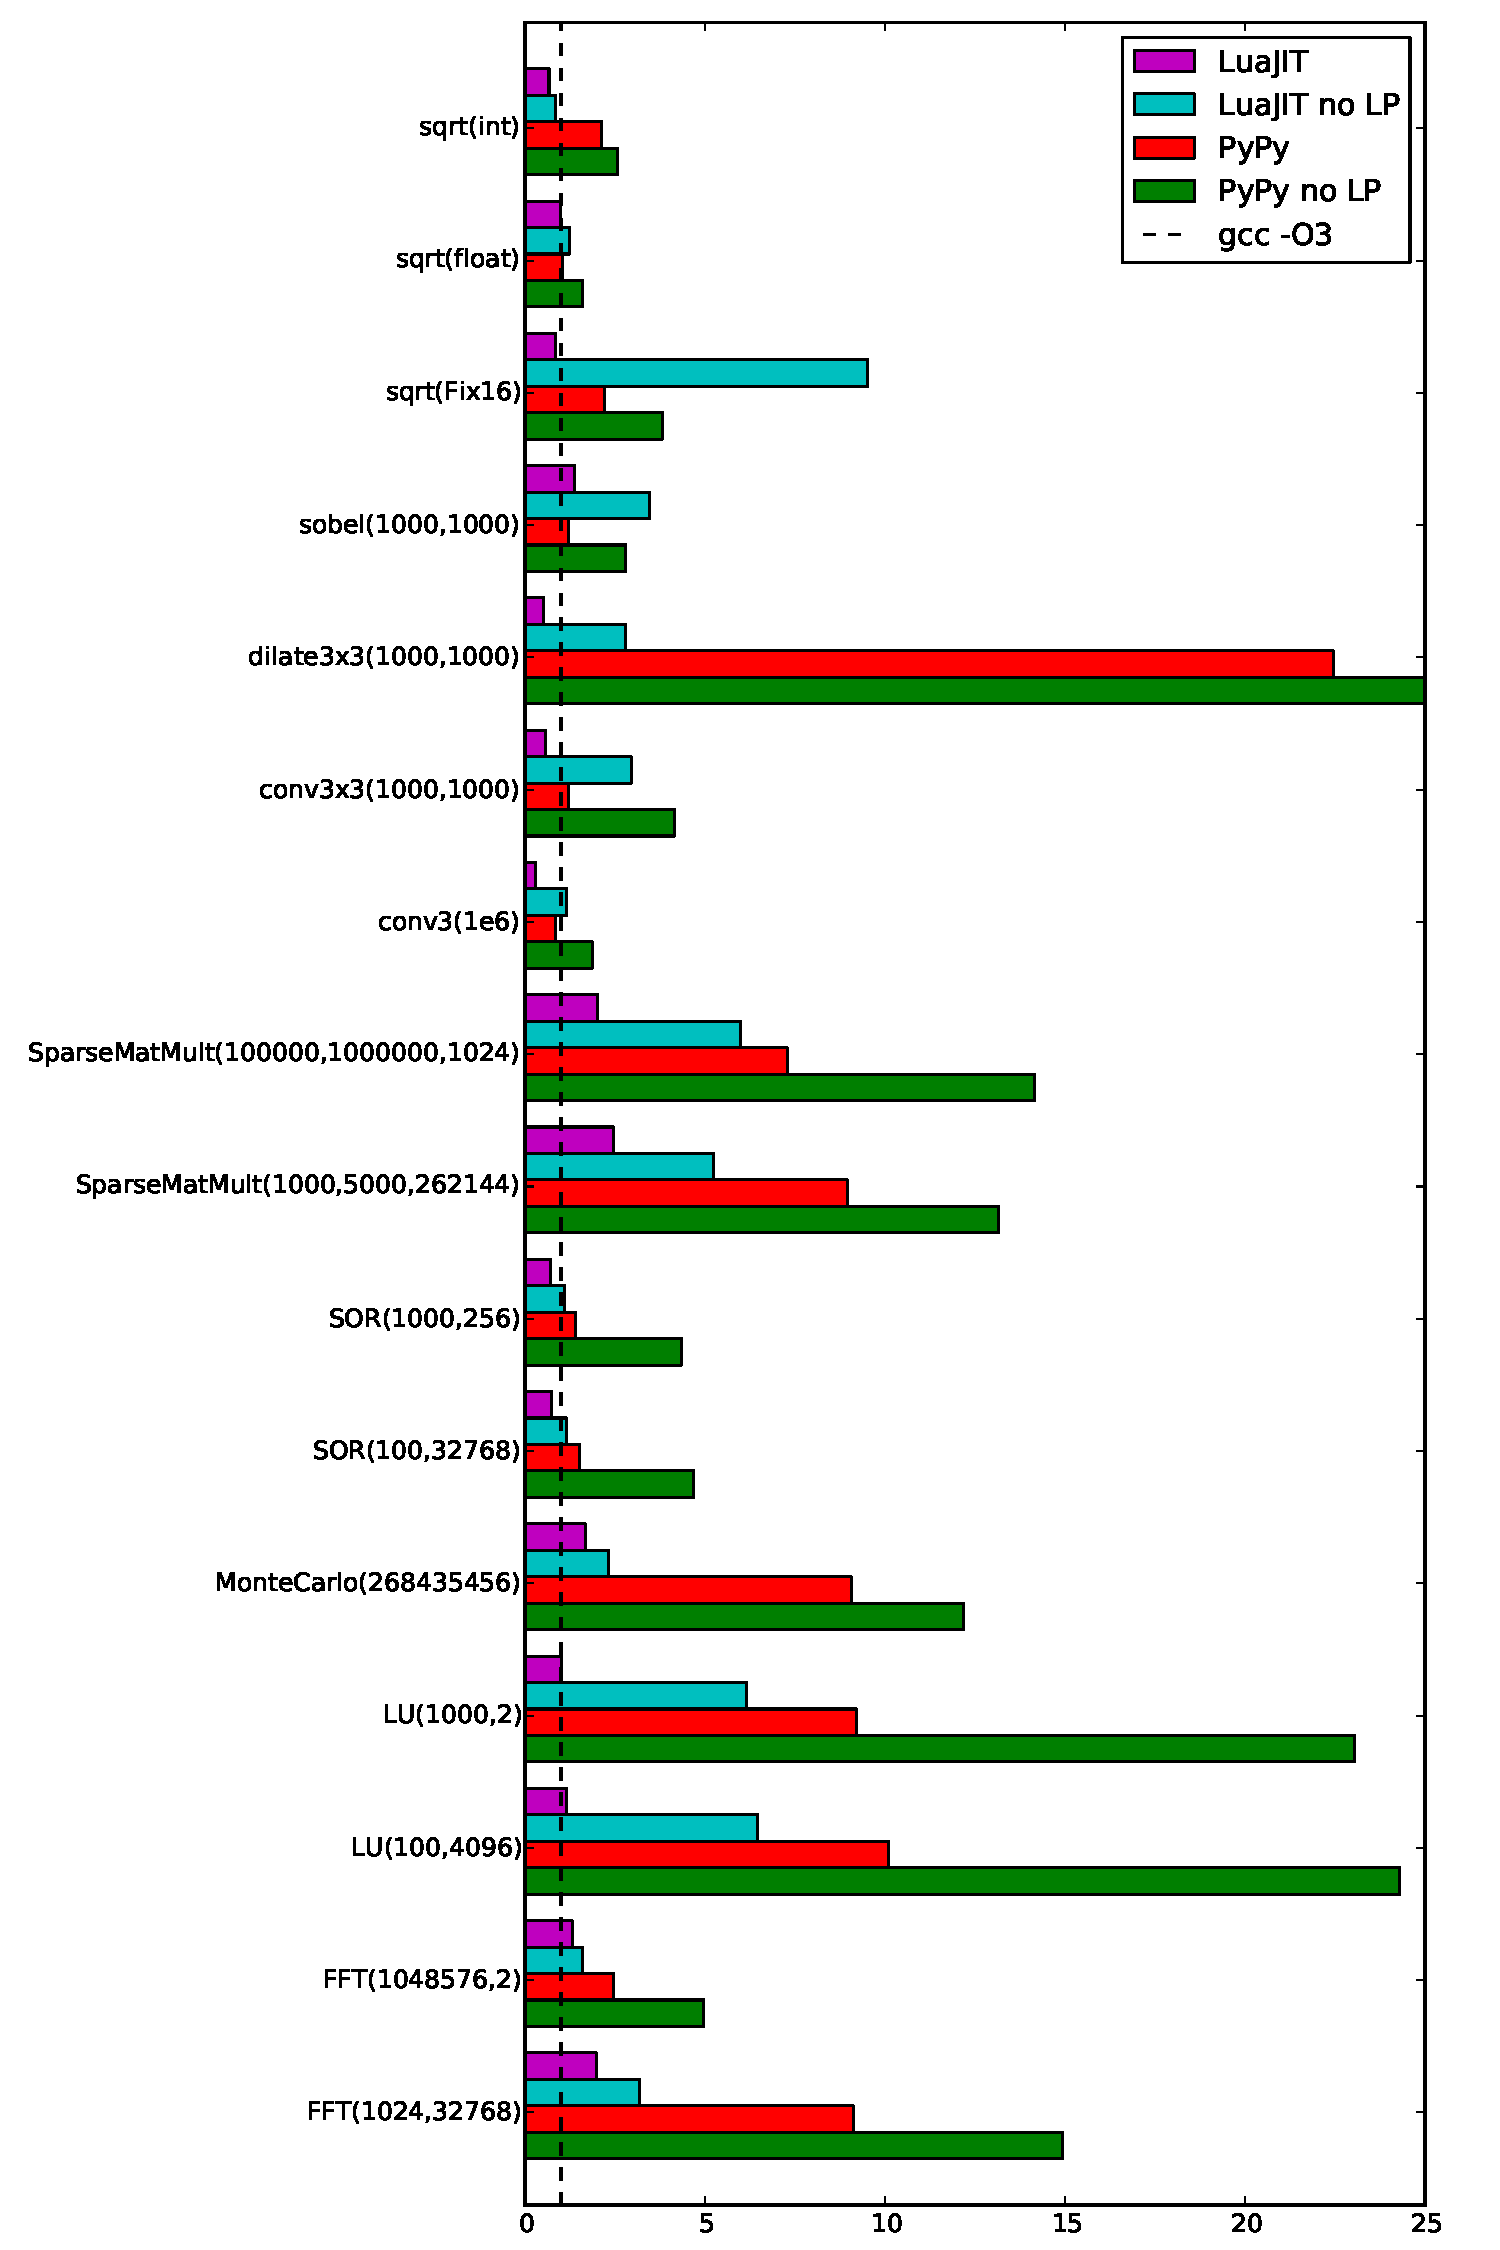
\includegraphics[width=0.5\textwidth]{benchmarks/result}
\end{center}
\caption{Benchmark results normalized to the runtime of the C version. The CPython results have been omitted to make the plot readable.}
\label{fig:benchmarks_plot}
\end{figure}

The Python interpreter of the RPython framework is a complete Python
version 2.7 compatible interpreter. A set of numerical
calculations were implemented in both Python, C and Lua and their
runtimes are compared in Figure~\ref{fig:benchmarks_plot} and Figure~\ref{fig:benchmarks}.\footnote{
    The benchmarks and the scripts to run them can be found in the repository for this paper:
    \texttt{https://bitbucket.org/pypy/extradoc/src/ tip/talk/dls2012/benchmarks}
}
For benchmarks using larger Python applications the times are unaffected or
only slightly improved by the loop optimization of this paper.

The benchmarks are
\begin{itemize}
\item {\bf conv3}$\left(n\right)$: one-dimensional convolution with fixed kernel-size $3$. A single loop
is used to calculate a vector ${\bf b} = \left(b_1, \cdots, b_{n-2}\right)$ from a vector
${\bf a} = \left(a_1, \cdots, a_n\right)$ and a kernel ${\bf k} = \left(k_1, k_2, k_3\right)$ using 
$b_i = k_3 a_i + k_2 a_{i+1} + k_1 a_{i+2}$ for $1 \leq i \leq n-2$. Both the output vector, $\bf b$, 
and the input vectors, $\bf a$ and $\bf k$, are allocated prior to running the benchmark. It is executed 
with $n=10^5$.
%\item {\bf conv5}$\left(n\right)$: one-dimensional convolution with fixed kernel-size $5$. Similar to conv3, but with 
%${\bf k} = \left(k_1, k_2, k_3, k_4, k_5\right)$. The enumeration of the elements in $\bf k$ is still 
%hardcoded into the implementation making the benchmark consist of a single loop too.
\item {\bf conv3x3}$\left(n,m\right)$: two-dimensional convolution with a kernel of fixed
  size $3 \times 3$ using a custom class to represent two-dimensional
  arrays. It is implemented as two nested loops that iterates over the elements of the 
$m\times n$ output matrix ${\bf B} = \left(b_{i,j}\right)$ and calculates each element from the input matrix
${\bf A} = \left(a_{i,j}\right)$ and a kernel ${\bf K} = \left(k_{i,j}\right)$ using $b_{i,j} = $
\begin{equation}
  \label{eq:convsum}
  \begin{array}{lclclc}
    k_{3,3} a_{i-1,j-1} &+& k_{3,2} a_{i-1,j} &+& k_{3,1} a_{i-1,j+1} & + \\
    k_{2,3} a_{i,j-1}   &+& k_{2,2} a_{i,j}   &+& k_{2,1} a_{i,j+1}   & + \\
    k_{1,3} a_{i+1,j-1} &+& k_{1,2} a_{i+1,j} &+& k_{1,1} a_{i+1,j+1}  \\
  \end{array}
\end{equation}
for $2 \leq i \leq m-1$ and $2 \leq j \leq n-1$.
The memory for storing the matrices are again allocated outside the benchmark and $(n,m)=(1000,1000)$ 
 was used.
\item {\bf dilate3x3}$\left(n\right)$: two-dimensional dilation with a kernel of fixed
  size $3 \times 3$. This is similar to convolution but instead of
  summing over the terms in Equation~\ref{eq:convsum}, the maximum over those terms is taken. That places a
  external call to a max function within the loop that prevents some
  of the optimizations for PyPy.
\item {\bf sobel}$\left(n\right)$: a low-level video processing algorithm used to
  locate edges in an image. It calculates the gradient magnitude
  using sobel derivatives. A Sobel x-derivative, $D_x$, of a $n \times n$ image, ${I}$, is formed
by convolving ${I}$ with
\begin{equation}
  {K} = \left(
  \begin{array}{ccc}
    -1 & 0 & 1 \\
    -2 & 0 & 2 \\
    -1 & 0 & 1 \\
  \end{array}
  \right) ,
\end{equation}
and a Sobel y-derivative, $D_y$, is formed convolving $I$ with $K^\top$. The gradient magnitude is 
then formed for each pixel independently by $\sqrt{D_x^2 + D_y^2}$. The two convolutions and the pixelwise
magnitude calculation are combined in the implementation of this benchmark and calculated in a single pass over
the input image. This single pass consists of two nested loops with a somewhat larger amount of calculations 
performed each iteration as compared to the other benchmarks.

\item {\bf sqrt}$\left(T\right)$: approximates the square root of $y$. The approximation is 
initialized to $x_0=y/2$ and the benchmark consists of a single loop updating this
approximation using $x_i = \left( x_{i-1} + y/x_{i-1} \right) / 2$ for $1\leq i < 10^8$. 
Only the latest calculated value $x_i$ is kept alive as a local variable within the loop.
There are three different versions of this benchmark where $x_i$
  is represented with different type $T$ of objects: int's, float's and
  Fix16's. The latter, Fix16, is a custom class that implements
  fixpoint arithmetic with 16 bits precision. In Python and Lua there is only
  a single implementation of the benchmark that gets specialized
  depending on the class of it's input argument, $y$. In C,
  there are three different implementations.

The Fix16 type is a custom class with operator overloading in Lua and Python.
The C version uses a C++ class. The goal of this variant of the benchmark is to
check how large the overhead of a custom arithmetic class is, compared to
builtin data types.

In Lua there is no direct support for
integers so the int version is not provided.

\end{itemize}

The sobel and conv3x3 benchmarks are implemented
on top of a custom two-dimensional array class.
It is
a straightforward implementation providing 2 dimensional
indexing with out of bounds checks and 
data stored in row-major order.
For the C implementations it is
implemented as a C++ class. The other benchmarks are implemented in
plain C. All the benchmarks except sqrt operate on C double-precision floating
point numbers, both in the Python, C and Lua code.

In addition we also ported the 
SciMark\footnote{\texttt{http://math.nist.gov/scimark2/}} benchmarts to Python, and compared
their runtimes with the already existing
Lua\footnote{\texttt{http://luajit.org/download/scimark.lua}} and C
implementations.

SciMark consists of:

\begin{itemize}
\item {\bf FFT}$\left(n, c\right)$: Fast Fourier Transform of a vector with $n$ elements, represented as an array, repeated $c$ times.
\item {\bf LU}$\left(n, c\right)$: LU factorization of an $n \times n$ matrix. The rows of the matrix is shuffled which makes the previously used two-dimensional array class unsuitable. Instead a list of arrays is used to represent the matrix. The calculation is repeated $c$ times.
\item {\bf MonteCarlo}$\left(n\right)$: Monte Carlo integration by generating $n$ points uniformly distributed over the unit square and computing the ratio of those within the unit circle.
\item {\bf SOR}$\left(n, c\right)$: Jacobi successive over-relaxation on a $n\times n$ grid repreated $c$ times.
The same custom two-dimensional array class as described above is used to represent
the grid.
\item {\bf SparseMatMult}$\left(n, z, c\right)$: Matrix multiplication between a $n\times n$ sparse matrix,
stored in compressed-row format, and a full storage vector, stored in a normal array. The matrix has $z$ non-zero elements and the calculation is repeated $c$ times.
\end{itemize}

Benchmarks were run on Intel Xeon X5680 @3.33GHz with 12M cache and 16G of RAM
using Ubuntu Linux 11.4 in 64bit mode.
The machine was otherwise unoccupied. We used the following software
for benchmarks:

\begin{itemize}
\item PyPy 1.9
\item CPython 2.7.1
\item GCC 4.5.2 shipped with Ubuntu 11.4
\item LuaJIT 2.0 beta, git head of August 15, 2012, commit ID 0dd175d9
\end{itemize}

We ran GCC with -O3 -march=native, disabling the
automatic loop vectorization. In all cases, SSE2 instructions were used for
floating point operations.
We also ran PyPy and LuaJIT with loop peeling optimization and without (but otherwise
identical).

For PyPy and LuaJIT, 10 iterations were run, prefaced with 3 iterations for warming up.
Due to benchmarks taking large amounts of time on CPython, only one run
was performed.
For GCC, 5 iterations
were run. In all cases, the standard deviation is very low, making benchmarks
very well reproducible.

We can observe that PyPy (even without loop peeling) is orders of magnitude
faster than CPython. This is due to the JIT compilation
advantages and optimizations we discussed in previous
work~\cite{bolz_allocation_2011, bolz_runtime_2011}, the main improvement for
these concrete benchmarks comes from the allocation removal/unboxing
optimization.

The geometric mean of the
speedup of loop peeling is 70\%, which makes benchmark times
comparable with native-compiled C code. We attribute the performance gap to C code to
the relative immaturity of RPython's JIT machine code backend and the naive register allocator.
Also, in case of nested loops,
operations are only moved out of the 
innermost loop. That is an issue when the innermost loop is 
short and a significant amount of time is spent in the outer loops. This is the case 
with for example SparseMatMult.

The large input parameters of the SciMark benchmarks are chosen in such a way
to make the problem not fit into the CPU cache. This explains why PyPy is doing
relatively better on them. The cache miss penalties are large relative to the
time needed to perform the actual computations, which hides problems of the
less efficient code generated by PyPy.

The speedups that LuaJIT gains from the loop optimization pass are similar to
those PyPy gains. In general, LuaJIT is even closer to C performance, sometimes
even surpassing it. LuaJIT is generating machine code of higher quality because
it has more optimizations\footnote{See
\texttt{http://wiki.luajit.org/Optimizations}} and produces much better
machine code than PyPy.

The performance of sqrt(Fix16) compared to the C version gives an indication of the
overhead of using a custom class with operator overloading for arithmetic. For
CPython the overhead over C is a lot larger than that of sqrt(int).
In LuaJIT, the overhead is very small. For PyPy, sqrt(Fix16) 2.2 times slower
than the C version. However, that is not actually due to the overhead of
operator overloading but due to the additional overflow checking necessary
for integer arithmetic in Python. The JIT does not manage to prove that the
integer operations in these benchmarks cannot overflow and therefore cannot
optimize away the overflow checking. This is also the reason why sqrt(float) is
so much faster than sqrt(int) for PyPy.
The fact that LuaJIT and PyPy do so well on
sqrt(Fix16) shows that the allocation removal/sinking optimizations work well
in both JITs.

\section{Related Work}
\label{sec:related}

Loop invariant code motion optimizations are a well-known approach to optimize
loops~\cite{muchnick_advanced_1997}. Therefore, the effects that the
optimizations described here achieve are not in any way new. However, we think
that achieving them in the way described in this paper is simpler than writing
explicit algorithms.

Loop invariant code motion has been part of early compilers since the
1960s~\cite{allen_catalogue_1971}. A common approach for achieving loop
invariant
code motion is to perform partial redundancy elimination. The
approach was first proposed by Morel and Renvoise~\cite{morel_global_1979}. It
involves solving data flow problems of bidirectional data flow
equations. After improvements~\cite{chow_portable_1984,
dhamdhere_practical_1991} this approach was followed by the work of Knoop
et.al.~\cite{knoop_lazy_1992} who cleanly separated the problem into a backward
and forward data flow analysis. Implementing partial redundancy elimination in
compilers that use SSA form~\cite{chow_new_1997} simplified the algorithms,
because no iterative data flow analysis was needed any more.

As described in the introduction,
Mike Pall pioneered the approach described in this paper.
He showed that, unlike traditional loop-invariant code motion
(LICM), this approach is effective, even in the presence of many
guards and global control dependencies, which are caused by the
semantics of dynamic languages.

He writes on the Lua-users mailing list:
``The LOOP pass does synthetic unrolling of the recorded IR, combining
copy-substitution with redundancy elimination to achieve code hoisting. The
unrolled and copy-substituted instructions are simply fed back into the
compiler pipeline, which allows reuse of all optimizations for redundancy
elimination. Loop recurrences are detected on-the-fly and a minimized set of
PHIs is generated.''~\cite{pall_luajit_2009}

Both the Hotpath VM~\cite{gal_hotpathvm:_2006} and
SPUR~\cite{bebenita_spur:_2010} implement loop-invariant code motion
directly, by explicitly marking as loop-invariant all variables that stay the
same along all looping paths and then moving all pure computation that depends
only on these variables out of the loop. SPUR can also hoist loads out of the
loop if nothing in the loop can ever write to the memory location. It can also
move allocations out of the loop, but does not replace the object by its attributes.
This saves only the allocation, not the access to the object attributes.

The type specialization described by Gal \etal~\cite{gal_trace-based_2009} can
be seen as doing a similar optimization (again by manually implementing it)
as the one described in Section~\ref{sub:allocation}: The effect of both is
that type checks are fully done before a loop is even entered.


% section Related Work (end)

\section{Conclusions}

In this paper we have studied loop invariant code motion during trace
compilation. We claim that the loop peeling approach of LuaJIT is a very convenient solution
since it fits well with other trace optimizations and does not require
large changes to them. The approach improves the effect of standard
optimizations such as redundant guard removal, common subexpression elimination
and allocation removal. The most prominent effect is that they all become loop
invariant code motion optimizations.

By using several benchmarks we show that the proposed algorithm can
significantly improve the run time of small loops containing numerical
calculations.

The described approach still has some limitations which we plan to address in the
future. In particular loop peeling works poorly in combination with trace
trees~\cite{gal_incremental_2006} or trace stitching~\cite{gal_trace-based_2009}.
The side exits attached to guards that fail often
currently have to jump to the preamble.

%\appendix
%\section{Appendix Title}

%This is the text of the appendix, if you need one.

\acks
We would like to thank Samuele Pedroni, Sven Hager, David Schneider, and the anonymous reviewers
for helpful comments on drafts of this paper. We owe gratitude to Mike Pall
for making his impressive work on LuaJIT publicly available and for detailed
reviews on drafts of the paper.

% We recommend abbrvnat bibliography style.

\bibliographystyle{abbrv}
\bibliography{paper}

\end{document}
